\documentclass{article}
\usepackage[utf8]{inputenc}
\usepackage[T1]{fontenc}
\usepackage{graphicx}
\usepackage{color}

\newenvironment{text-blue}{\color{blue}}{}
\newenvironment{text-red}{\color{red}}{}


\begin{document}

\title{Monitorização da temperatura do ar de um processo térmico \\ Trabalho prático nº3, Computação Adaptativa}
\author{Adriano Vinhas (2009106560, avinhas@student.dei.uc.pt)\\
		José Ribeiro (2008112181, jbaia@student.dei.uc.pt}
\maketitle
\clearpage

% Introdução
\section{Introdução}

\indent \indent Este trabalho, no âmbito da disciplina de Computação Adaptativa, tem como objectivo construir um sistema difuso capaz de regular a temperatura do ar através de um conjunto de entradas facultadas à rede, sendo estas alvo de transformação para corresponderem à lógica difusa. Estes valores vão ser a base da decisão de uma acção a tomar pelo sistema, que é feita através da saída.

Este objectivo foi atingido fazendo um estudo paramétrico tendo em conta os seguintes parâmetros de estudo:
\begin{itemize}
\item Factor de normalização
\item Conjunto e número de termos linguísticos
\item Tipo de funções de pertença
\item Base de regras
\item Mecanismo de inferência
\item Método de desfuzificação
\end{itemize}

A parte que foi mais focada na realização deste trabalho foi o estudo paramétrico feito com base nos parâmetros acima indicados. Com base nos resultados obtidos, procurámos uma solução que nos permitisse chegar à combinação dos parâmetros que minimizasse o erro da rede, para as referências que nos foram fornecidas.

\clearpage
\section{Concepção da rede difusa}
\indent \indent Nesta secção estão descritas a arquitectura da rede usada para o trabalho bem como outras decisões tomadas que são relevantes para o desempenho do controlador.

A figura~\ref{nn_architecture} representa a arquitectura do sistema difuso usado.

\begin{figure}[!h]
  \centering
  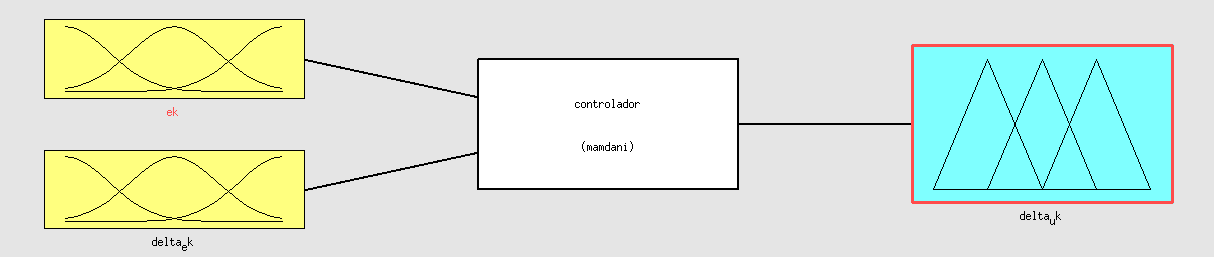
\includegraphics[width=5in]{figures/nn_architecture}
  \caption{Arquitectura da rede usada}
  \label{nn_architecture}
\end{figure}

\subsection{Entradas}
\indent \indent A arquitectura do sistema difuso usada para o trabalho prático consiste em duas entradas, uma delas que representa o erro num instante $k$ ($E$) como a diferença entre a temperatura desejada e a temperatura do ar à saída do aquecedor nesse mesmo instante ($E = R_{k} - Y_{k}$), e a outra representando a variação do erro ($\Delta E$) como a diferença entre o erro no instante $k$ e $k-1$ ($\Delta E=E_{k}-E_{k-1}$).

Relativamente ao \textbf{universo de discurso}, considerámos que a variável $E$, poderia tomar valores entre -50 e 50 e a variável $\Delta e$ tomaria valores entre -100 e 100.

Os valores de erro e variação de erro que serviram de entrada para o sistema de difuso foram alvo de normalização, de modo a mapear os valores de temperatura e potência para a gama de valores nas quais as funções de pertença estão definidas. Assim sendo, em relação aos \textbf{factores de normalização} utilizados, optámos por um usar um factor de escala de \textbf{0.02} para o erro e de \textbf{0.01} para a variação do erro, de modo a conseguir transformar o universo de discurso das variáveis em valores que variam entre -1 e 1  

Já para o caso da potência, à saída, aplicou-se um factor de escala de \textbf{100} para fazer a transformação contrária e mapear valores da saída, entre -1 e 1, para a gama de valores que a potência pode tomar (entre 0 e 100\%). 

%Em relação às saídas do sistema difuso, apenas foi definida uma, que representa a variação de potência a aplicar à grelha de aquecimento ($\Delta U$).

No que diz respeito às características das funções da pertença, foram consideradas 4 abordagens para a execução do estudo paramétrica:
\begin{itemize}
\item \textbf{Termos linguísticos}:(${N,ZO,P}$) e \textbf{Tipo de funções de pertença}: Triangulares
\item \textbf{Termos linguísticos}:(${N,ZO,P}$) e \textbf{Tipo de funções de pertença}: Gaussianas
\item \textbf{Termos linguísticos}:(${NG,NP,ZO,PP,PG}$) e \textbf{Tipo de funções de pertença}: Triangulares
\item \textbf{Termos linguísticos}:(${NG,NP,ZO,PP,PG}$) e \textbf{Tipo de funções de pertença}: Gaussianas
\end{itemize}

Cada uma das abordagens foi replicada para todas as variáveis linguísticas, enquanto que o \textit{offset} de cada função de pertença foi sempre o mesmo, independentemente da abordagem.
Cada uma destas está representada, respectivamente, pelas figuras~\ref{trimf_3}~\ref{gauss_3},~\ref{trimf_5} e ~\ref{gauss_5}.

\begin{figure}[!h]
  \centering
  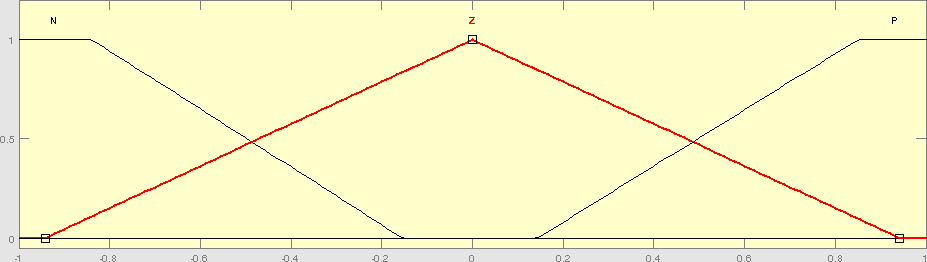
\includegraphics[width=3in]{figures/trimf3}
  \caption{3 termos linguísticos com funções de pertença tringulares}
  \label{trimf_3}
\end{figure}

\begin{figure}[!h]
  \centering
  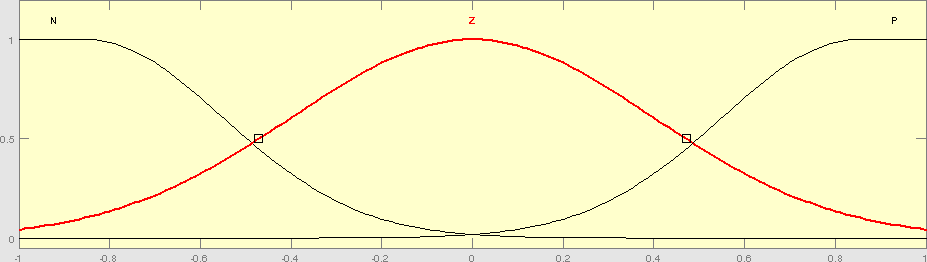
\includegraphics[width=3in]{figures/gauss3}
  \caption{3 termos linguísticos com funções de pertença gaussianas}
  \label{gauss_3}
\end{figure}

\begin{figure}[!h]
  \centering
  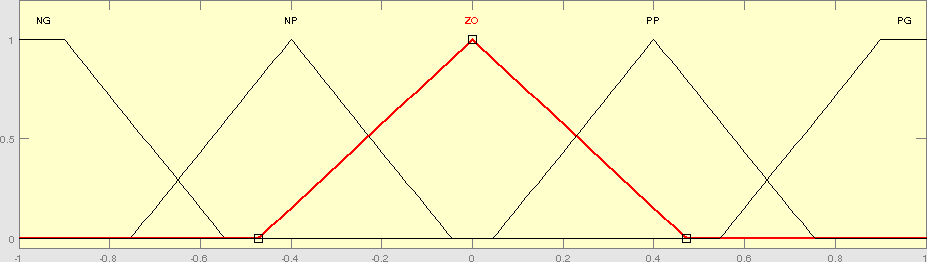
\includegraphics[width=3in]{figures/trimf5}
  \caption{5 termos linguísticos com funções de pertença tringulares}
  \label{trimf_5}
\end{figure}

\begin{figure}[!h]
  \centering
  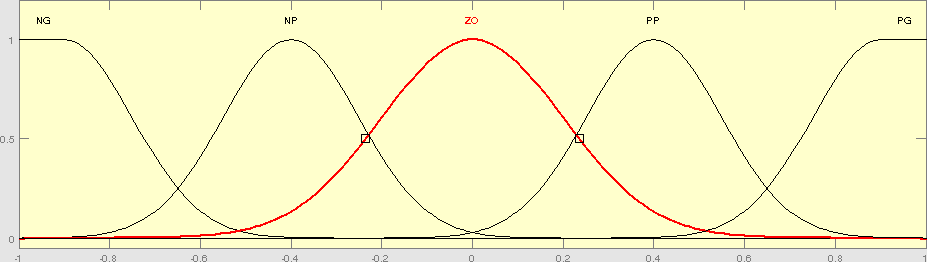
\includegraphics[width=3in]{figures/gauss5}
  \caption{5 termos linguísticos com funções de pertença gaussianas}
  \label{gauss_5}
\end{figure}

\subsection{Base de Regras}
\indent \indent O conjunto de regras que gerem as acções a tomar em função das entradas foi feito com especial cuidado uma vez que, entre outros factores, a definição das regras tem impacto na performance do sistema difuso.

Considerámos dois grupos distintos de controladores no que toca ao número de termos linguísticos considerados para as entradas e a saída: 3 e 5 termos. Descrevem-se em seguida as suas diferenças.

\subsection{Controlador de 3 termos}
\indent \indent Para este controlador existem as três variáveis linguísticas mencionadas acima ($E$,$\Delta E$,$\Delta U$) e cada uma destas variavéis tem três termos linguísticos (${N,Z,P}$).

A tabela de regras para este controlador está representada na tabela~\ref{3_terms_fuzzy}.

\begin{table}[!h]
\centering
	\caption{Tabela de regras do controlador difuso de 3 termos}
	\label{3_terms_fuzzy}
	\begin{tabular}{|c|c|c|c|}
	\hline
	$E$ $\backslash$ $\Delta E$ & \textbf{N} & \textbf{ZO} & \textbf{P} \\ 
	\hline 
	\textbf{N} & N & N & ZO \\ 
	\hline 
	\textbf{ZO} & ZO & ZO & ZO \\ 
	\hline 
	\textbf{P} & ZO & P & P \\ 
	\hline 
	\end{tabular} 
	%\vspace{-1cm}
\end{table}

Esta tabela traduz-se na seguinte lista de regras:
\begin{itemize}
	\item \texttt{IF} <E \texttt{is} N> \texttt{AND} <$\Delta E$ \texttt{is} N> \texttt{THEN} <$\Delta U$ \texttt{is} N>
	\item \texttt{IF} <E \texttt{is} N> \texttt{AND} <$\Delta E$ \texttt{is} ZO> \texttt{THEN} <$\Delta U$ \texttt{is} N>
	\item \texttt{IF} <E \texttt{is} N> \texttt{AND} <$\Delta E$ \texttt{is} P> \texttt{THEN} <$\Delta U$ \texttt{is} ZO>
	\item \texttt{IF} <E \texttt{is} ZO> \texttt{AND} <$\Delta E$ \texttt{is} N> \texttt{THEN} <$\Delta U$ \texttt{is} ZO>
	\item \texttt{IF} <E \texttt{is} ZO> \texttt{AND} <$\Delta E$ \texttt{is} ZO> \texttt{THEN} <$\Delta U$ \texttt{is} ZO>
	\item \texttt{IF} <E \texttt{is} ZO> \texttt{AND} <$\Delta E$ \texttt{is} P> \texttt{THEN} <$\Delta U$ \texttt{is} ZO>
	\item \texttt{IF} <E \texttt{is} P> \texttt{AND} <$\Delta E$ \texttt{is} N> \texttt{THEN} <$\Delta U$ \texttt{is} ZO>
	\item \texttt{IF} <E \texttt{is} P> \texttt{AND} <$\Delta E$ \texttt{is} ZO> \texttt{THEN} <$\Delta U$ \texttt{is} P>
	\item \texttt{IF} <E \texttt{is} P> \texttt{AND} <$\Delta E$ \texttt{is} P> \texttt{THEN} <$\Delta U$ \texttt{is} P>
\end{itemize}

\clearpage

\subsection{Controlador de 5 termos}
\indent \indent Para este controlador existem as mesmas variáveis linguísticas e cada uma destas variavéis tem cinco termos linguísticos (${NG,NP,ZO,PP,PG}$).

A tabela de regras para este controlador está representada na tabela~\ref{5_terms_fuzzy}.

\begin{table}[!h]
\centering
	\caption{Tabela de regras do controlador difuso de 5 termos}
	\label{5_terms_fuzzy}
	\begin{tabular}{|c|c|c|c|c|c|}
	\hline
	$E$ $\backslash$ $\Delta E$ & \textbf{NG} & \textbf{NP} & \textbf{ZO} & \textbf{PP} & \textbf{PG} \\ 
	\hline 
	\textbf{NG} & NG & NG & NG & NP & NP \\ 
	\hline 
	\textbf{NP} & NP & NP & NP & NP & NG \\ 
	\hline 
	\textbf{ZO} & NP & ZO & ZO & ZO & PP \\ 
	\hline
	\textbf{PP} & PG & PP & PP & PP & PP \\ 
	\hline 
	\textbf{PG} & PP & PP & PG & PG & PG \\ 
	\hline 
	\end{tabular} 
	%\vspace{-1cm}
\end{table}

Esta tabela traduz-se na seguinte lista de regras:
\begin{itemize}
	\item \texttt{IF} <E \texttt{is} NG> \texttt{AND} <$\Delta E$ \texttt{is} NG> \texttt{THEN} <$\Delta U$ \texttt{is} NG>
	\item \texttt{IF} <E \texttt{is} NG> \texttt{AND} <$\Delta E$ \texttt{is} NP> \texttt{THEN} <$\Delta U$ \texttt{is} NG>
	\item \texttt{IF} <E \texttt{is} NG> \texttt{AND} <$\Delta E$ \texttt{is} ZO> \texttt{THEN} <$\Delta U$ \texttt{is} NG>
	\item \texttt{IF} <E \texttt{is} NG> \texttt{AND} <$\Delta E$ \texttt{is} PP> \texttt{THEN} <$\Delta U$ \texttt{is} NP>
	\item \texttt{IF} <E \texttt{is} NG> \texttt{AND} <$\Delta E$ \texttt{is} PG> \texttt{THEN} <$\Delta U$ \texttt{is} NP>
	\item \texttt{IF} <E \texttt{is} NP> \texttt{AND} <$\Delta E$ \texttt{is} NG> \texttt{THEN} <$\Delta U$ \texttt{is} NP>
	\item \texttt{IF} <E \texttt{is} NP> \texttt{AND} <$\Delta E$ \texttt{is} NP> \texttt{THEN} <$\Delta U$ \texttt{is} NP>
	\item \texttt{IF} <E \texttt{is} NP> \texttt{AND} <$\Delta E$ \texttt{is} ZO> \texttt{THEN} <$\Delta U$ \texttt{is} NP>
	\item \texttt{IF} <E \texttt{is} NP> \texttt{AND} <$\Delta E$ \texttt{is} PP> \texttt{THEN} <$\Delta U$ \texttt{is} NP>
	\item \texttt{IF} <E \texttt{is} NP> \texttt{AND} <$\Delta E$ \texttt{is} PG> \texttt{THEN} <$\Delta U$ \texttt{is} NG>
	\item \texttt{IF} <E \texttt{is} ZO> \texttt{AND} <$\Delta E$ \texttt{is} NG> \texttt{THEN} <$\Delta U$ \texttt{is} NP>
	\item \texttt{IF} <E \texttt{is} ZO> \texttt{AND} <$\Delta E$ \texttt{is} NP> \texttt{THEN} <$\Delta U$ \texttt{is} ZO>
	\item \texttt{IF} <E \texttt{is} ZO> \texttt{AND} <$\Delta E$ \texttt{is} ZO> \texttt{THEN} <$\Delta U$ \texttt{is} ZO>
	\item \texttt{IF} <E \texttt{is} ZO> \texttt{AND} <$\Delta E$ \texttt{is} PP> \texttt{THEN} <$\Delta U$ \texttt{is} ZO>
	\item \texttt{IF} <E \texttt{is} ZO> \texttt{AND} <$\Delta E$ \texttt{is} PG> \texttt{THEN} <$\Delta U$ \texttt{is} PP>
	\item \texttt{IF} <E \texttt{is} PP> \texttt{AND} <$\Delta E$ \texttt{is} NG> \texttt{THEN} <$\Delta U$ \texttt{is} PG>
	\item \texttt{IF} <E \texttt{is} PP> \texttt{AND} <$\Delta E$ \texttt{is} NP> \texttt{THEN} <$\Delta U$ \texttt{is} PP>
	\item \texttt{IF} <E \texttt{is} PP> \texttt{AND} <$\Delta E$ \texttt{is} ZO> \texttt{THEN} <$\Delta U$ \texttt{is} PP>
	\item \texttt{IF} <E \texttt{is} PP> \texttt{AND} <$\Delta E$ \texttt{is} PP> \texttt{THEN} <$\Delta U$ \texttt{is} PP>
	\item \texttt{IF} <E \texttt{is} PP> \texttt{AND} <$\Delta E$ \texttt{is} PG> \texttt{THEN} <$\Delta U$ \texttt{is} PP>
	\item \texttt{IF} <E \texttt{is} PG> \texttt{AND} <$\Delta E$ \texttt{is} NG> \texttt{THEN} <$\Delta U$ \texttt{is} PP>
	\item \texttt{IF} <E \texttt{is} PG> \texttt{AND} <$\Delta E$ \texttt{is} NP> \texttt{THEN} <$\Delta U$ \texttt{is} PP>
	\item \texttt{IF} <E \texttt{is} PG> \texttt{AND} <$\Delta E$ \texttt{is} ZO> \texttt{THEN} <$\Delta U$ \texttt{is} PG>
	\item \texttt{IF} <E \texttt{is} PG> \texttt{AND} <$\Delta E$ \texttt{is} PP> \texttt{THEN} <$\Delta U$ \texttt{is} PG>
	\item \texttt{IF} <E \texttt{is} PG> \texttt{AND} <$\Delta E$ \texttt{is} PG> \texttt{THEN} <$\Delta U$ \texttt{is} PG>
\end{itemize}

\clearpage

\subsection{Método de Implicação e Agregação de Regras}
\indent \indent Após a aplicação do \textit{fuzzy operator} e obtido o valor de verdade para o antecedente de cada regra, é necessário calcular o conjunto difuso correspondente a cada variável de saída usando esse valor, por regra. Uma das funções mais utilizadas neste processo é a função de \textbf{mínimo} (\texttt{min}), mas existem outras (nomeadamente a de \textbf{produto algébrico}, \texttt{prod}).

Obtidos os conjuntos difusos por varíavel de saída por regra, surge a necessidade de agregar esses conjuntos num único conjunto difuso, naquilo que se denomina Agregação. Uma das funções mais utilizadas neste processo é a função de \textbf{máximo} (\texttt{max}); no entanto, são também utilizadas outras como a \textbf{soma algébrica} (\texttt{sum}) ou o \textbf{OR probabilístico} (\texttt{probor}).

Para o nosso estudo paramétrico, decidimos definir dois conjuntos de funções a utilizar para as operações de \texttt{AND}, \texttt{OR}, \texttt{Implicação} e \texttt{Agregação}, como se apresenta na tabela~\ref{and_or_imp_agg_table}.

\begin{table}[!h]
\centering
	\caption{Tabela de funções utilizadas para as operações de \texttt{AND}, \texttt{OR}, \texttt{Implicação} e \texttt{Agregação}.}
	\label{and_or_imp_agg_table}
	\begin{tabular}{|c|c|c|c|c|c|}
	\hline
	Function set & \texttt{AND} & \texttt{OR} & \texttt{IMP} & \texttt{AGG} \\
	\hline 
	\texttt{zadeh} & \texttt{min} & \texttt{max} & \texttt{min} & \texttt{max} \\ 
	\hline 
	\texttt{algebraic} & \texttt{prod} & \texttt{probor} & \texttt{prod} & \texttt{sum} \\ 
	\hline 
	\end{tabular} 
	%\vspace{-1cm}
\end{table}

\subsection{Desfuzificação}
\indent \indent Para obter o valor final de variação de potência a induzir ao aquecedor, o conjunto difuso obtido após a fase agregação tem de ser desfuzificado, isto é, convertido num valor crespo.

Para este processo, vários métodos são usados como o cálculo do centróide (\texttt{centroid}), a bissectriz (\texttt{bisector}) ou o menor/médio/maior dos máximos (\texttt{SOM}/\texttt{MOM}/\texttt{LOM}).

Nos testes levados a cabo foram considerados os métodos de \texttt{centroid} e \texttt{bisector}.

\clearpage
% Gráficos com os resultados. Análise e interpretação.
\section{Resultados}
\indent \indent Nesta secção são apresentados os resultados obtidos, bem como as interpretações que se podem fazer a partir destes.

A execução de cada teste foi repetida 30 vezes de forma a obter a média do critério de erro, bem como o desvio-padrão.

O critério de erro utilizado pode ser calculando recorrendo à fórmula:
\[
	E = \frac{\displaystyle \sum_{k = 1}^{N}{(r_{k} - y_{k})^2} + \displaystyle \sum_{k = 1}^{N}{(u_{k} - u_{k-1})^2}}{N}
\]

De seguida são apresentados os resultados obtidos.
\begin{table}[!h]
\centering
	\caption{Tabela de regras do controlador difuso de 5 termos}
	\label{results}
	\begin{tabular}{|c|c|c|c|c|c|}
		\hline 
		\textbf{Nº de termos} & \textbf{Funções} & \textbf{Operadores} & \textbf{Desfuzificação} & \textbf{Média} & \textbf{Desvio-Padrão} \\
		\hline
		3 terms & \texttt{trimf} & \texttt{algebraic} & \texttt{centroid} & 86.627 & 3.624 \\
		\hline
		3 terms & \texttt{trimf} & \texttt{algebraic} & \texttt{bisector} & 83.846 & 2.199 \\
		\hline
		3 terms & \texttt{trimf} & \texttt{zadeh} & \texttt{centroid} & 74.824 & 0.593 \\
		\hline
		3 terms & \texttt{trimf} & \texttt{zadeh} & \texttt{bisector} & 74.204 & 0.652 \\
		\hline
		3 terms & \texttt{gauss} & \texttt{algebraic} & \texttt{centroid} & 73.320 & 0.499 \\
		\hline
		3 terms & \texttt{gauss} & \texttt{algebraic} & \texttt{bisector} & 85.331 & 3.419 \\
		\hline
		3 terms & \texttt{gauss} & \texttt{zadeh} & \texttt{centroid} & 73.121 & 0.574 \\
		\hline
		3 terms & \texttt{gauss} & \texttt{zadeh} & \texttt{bisector} & 73.377 & 0.464 \\
		\hline
		5 terms & \texttt{trimf} & \texttt{algebraic} & \texttt{centroid} & 107.419 & 0.79 \\
		\hline
		5 terms & \texttt{trimf} & \texttt{algebraic} & \texttt{bisector} & 108.633 & 1.591 \\
		\hline
		5 terms & \texttt{trimf} & \texttt{zadeh} & \texttt{centroid} & 103.604 & 0.813 \\
		\hline
		5 terms & \texttt{trimf} & \texttt{zadeh} & \texttt{bisector} & 104.01 & 1.747 \\
		\hline
		5 terms & \texttt{gauss} & \texttt{algebraic} & \texttt{centroid} & 100.416 & 0.516 \\
		\hline
		5 terms & \texttt{gauss} & \texttt{algebraic} & \texttt{bisector} & 114.191 & 0.947 \\
		\hline
		5 terms & \texttt{gauss} & \texttt{zadeh} & \texttt{centroid} & 93.625 & 0.525 \\
		\hline
		5 terms & \texttt{gauss} & \texttt{zadeh} & \texttt{bisector} & 106.071 & 1.7 \\
		\hline
	\end{tabular} 
	%\vspace{-1cm}
\end{table}

\clearpage
\section{Conclusão}
\indent \indent Depois do estudo paramétrico efectuado o sistema difuso que obteve melhores resultados tinha um valor de erro/critério de \textbf{xxx}, para a entrada que nos foi fornecida para efeitos de avaliação.

Atingimos estes valores usando a seguinte parametrização:
\begin{itemize}
\item Factor de normalização: \textbf{0.02} para $E$, \textbf{0.01} para $\Delta E$, \textbf{100} para $\Delta U$
\item Número de termos linguísticos: \textbf{3}
\item Tipo de funções de pertença: %\textbf{Gaussianas}
\item Base de regras: \textbf{Ver tabela~\ref{3_terms_fuzzy}}
\item Mecanismo de inferência: % \textbf{zadeh}
\item Método de desfuzificação: %\textbf{centroid}
\end{itemize}

O gráfico que representa os valores da referência, temperatura e controlo, para o melhor sistema difuso obtido, está exibido na figura ~\ref{best_fuzzy_results}. Os valores de entrada que nos foram fornecidos tiveram em conta um intervalo de tempo de 10 segundos e um intervalo de amostragem de 0.1s.

%\begin{figure}[h!]
%  \centering
%  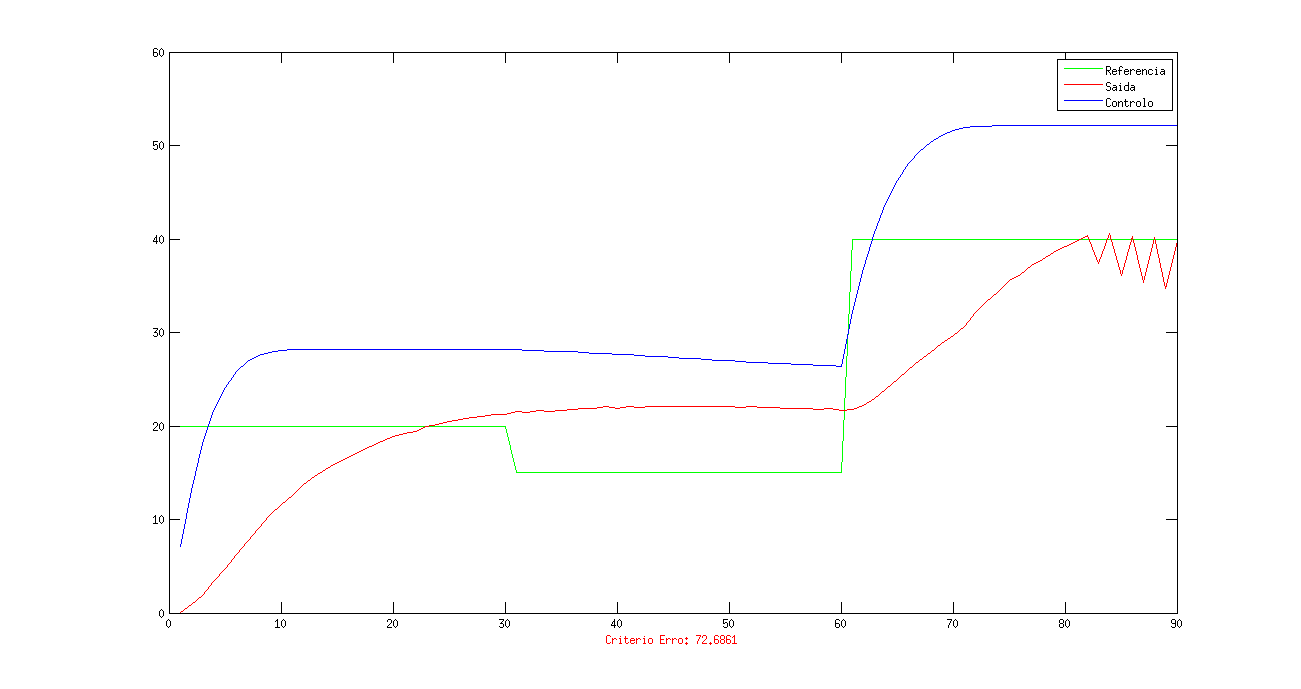
\includegraphics[width=5in]{figures/best_fuzzy_network}
%  \caption{Valores de Referência, Temperatura e potência para a melhor rede difusa}
%   \label{best_fuzzy_network}
%\end{figure}


\end{document}
